\documentclass[a4paper,12pt]{article}


\usepackage{amsmath}
\usepackage{graphicx}
\usepackage[capposition=bottom]{floatrow}
\usepackage{amssymb}
\usepackage{graphicx}
\usepackage{caption}
\usepackage{rotating}

\begin{document}
\title{Triated Methane as an Internal Calibration Source in Dark Matter Detectors}
\author{Richard Knoche}
\maketitle

\begin{abstract}
This paper provides an introduction to the cosmological evidence for dark matter, and briefly discusses the particle physics theories which seek to explain this evidence.  It then discusses terrestrial WIMP detection experiments with a focus on the Large Underground Xenon detector (LUX).  Details of the LUX experiment's effort to develop an internal calibration source for use in xenon detectors are included, and the results of R\&D projects to meet this goal are presented.
\end{abstract}

\tableofcontents



\section{Introduction to Dark Matter}

In recent decades it has been discovered that the luminous matter which scientists have studied for centuries is only a small fraction of the total composition of the universe.  There is strong evidence of dark baryonic matter (a few percent), nonbaryonic hot dark matter ($\sim$0.1\%-1.5\%), non baryonic cold dark matter ($\sim$25\%), and dark energy ($\sim$70\%) components to the universe, where the percentages are as a total fraction of their contribution to the universe's total composition.  While we know a large amount about the "normal" matter which contributes $ \lesssim $ 4\% of the universe's total composition, we know very little about these larger components.  In particular, while we understand certain characteristics of the cold dark matter component, there is no consensus on its composition.  Before examining the experiments which seek to answer this question we will first discuss what is currently known about the nonbaryonic dark matter component.

\subsection{Evidence of Dark Matter}

In the early 1930's Fritz Zwicky measured the rotational velocity of eight galaxies in the Coma Cluster.  Newtonian physics predicts that these rotational velocities will be given by $v(r)=\sqrt{GM(r)/r}$, where $M(r)$ is the mass enclosed by the orbit and G is Newton's gravitational constant.  In his examination, Zwicky found that the velocities at large radii were too high to be consistent with the Newtonian prediction arising from the visible matter alone \cite{Zwicky}. This discrepancy was reinforced in the 1970's, when further data on the rotational velocity of spiral galaxies began to be collected.  Instead of the rotational velocity falling off as $\propto 1/\sqrt{r}$ beyond the radius of visible matter as one would expect, the rotational velocity rises for small radii, then asymptotes to a constant $ v \simeq 100-300 km/s $ for large radii in most galaxies \cite{Persic,Battaner,Binney}.  The most widely accepted explanation of this phenomenon is that the disk galaxies are immersed in a dark matter (DM) halo such that $ M(r)/r $ remains constant at large radii.  Such a halo could form from a self gravitating ball of ideal gas at a uniform temperature.

\begin{center}
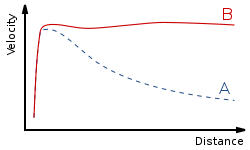
\includegraphics[scale=1]{RotationCurve.png}
\captionof{figure}{Rotation curve of a spiral galaxy.  The blue line (A) indicates the rotational velocity predicted by Newtonian physics when luminous matter alone is taken into acount.  The red line (B) indicates true rotational velocity seen from observations.}
\end{center}

To further examine the properties of these dark matter halos it is useful to introduce a quantitative measure for the composition of the universe.  Friedmann's equation, which describes the expansion of space in a homogeneous and isotropic universe, is given by
\[\frac{\dot{a}^2 + kc^2}{a^2} = \frac{8 \pi G \rho + \Lambda c^2}{3},\]
where $a$ is the scale factor of the universe, $k$ is the spatial curvature of the universe (equivalent to one sixth of the Ricci Scalar) , $c$ is the speed of light, $G$ is the gravitational constant, $\rho$ is the density of the universe, and $\Lambda$ is the cosmological constant. Einstein's field equations,
\[G_{\mu\nu} = \frac{8 \pi G}{c^4} T_{\mu\nu}\]
provide an expression for the cosmological constant, $\Lambda$.  We can split the stress energy tensor into two terms, one describing matter and the other describing the vacuum, such that $T_{\mu\nu}=T_{\mu\nu}^{matter}+T_{\mu\nu}^{vac}$.  Since the stress energy tensor is given by
\[T_{\mu\nu} = (\rho + p)U_{\mu}U_{\nu} + pg_{\mu\nu},\] 
and to maintain Lorentz invariance $p^{vac} = -\rho^{vac}$, we can write the vacuum component of the stress energy tensor as
\[T_{\mu\nu}^{vac}=-\rho^{vac} g_{\mu\nu}.\]
If we identify the vacuum energy density as
\[\rho^{vac}=\frac{\Lambda c^2}{8\pi G}\]
then Einstein's field equation takes on the familiar form
\[G_{\mu\nu} + g_{\mu\nu}\Lambda= \frac{8 \pi G}{c^4} T_{\mu\nu}^{matter},\]
where $G_{\mu\nu}$ is the Einstein tensor, $g_{\mu\nu}$ is the metric tensor, $G$ is the gravitational constant, and $\Lambda$ is the cosmological constant.
Setting the normalized spatial curvature $k = 0$ in Friedmann's equation(representing a flat universe), one can find the critical density for which the universe is spatially flat to be
\[\rho_c = \frac{3}{8 \pi G}\frac{\dot{a}^2}{a^2},\]
where $\rho_c = \rho^{vac}+\rho$.
Recognizing Hubble's constant to be $ H = \frac { \dot{a}}{a} $, we can rewrite this as
\[\rho_c =\frac{3H^2}{8 \pi G} \]
where $H$ is the present value of the Hubble constant \cite{Javorsek}. The current experimental value for $H$ in the dimensionless units 100 km/s/Mpc is $ h \sim 0.7 $ with an uncertainty of $\sim5\%$.  We can then define the density parameter as 
\[\Omega=\frac{\rho}{\rho_c}=\frac{8 \pi G \rho}{3 H_0^2}.\]
If $\Omega$ is larger than unity the universe is spatially closed, and if $\Omega$ is less than unity the universe is spatially open. This density parameter can be split into components, such that for a particular component $x$
\[\Omega_x = \frac{\rho_x}{\rho_c}.\]

Detailed cosmological studies have concluded that all the luminous matter in the universe has a density parameter of $\Omega_{lum} \lesssim 0.01$.  This information, combined  with the fact that analysis of galactic rotational velocities implies $> $90\% of the mass in galaxies is dark leads to the conclusion that $\Omega_{DM} \geq 0.09$.  This is only a lower limit on the dark matter density parameter, since most rotation curves remain flat out to the largest radii at which they can be measured and it can be assumed that the DM halos extend even further out.


With $\Omega_{DM} \geq 0.1$ it is possible that baryonic DM alone could be responsible for the dark halos.  However, other analyses eliminate this possibility. Direct searches for massive compact halo objects (MACHOs) utilizing microlensing have determined that $<$25\% of the dark halos could be due to baryonic dark matter within the mass range of $ 2 \times 10^{-7} M_{sun} < M < 1 M_{sun} $ at a 95\% confidence limit \cite{EROS,Alcock}. Furthermore, data from the Hubble Deep Field Space Telescope suggests dark matter halos consist of $\leq$5\% white dwarfs.

With baryonic dark matter being ruled out as the sole component of dark matter halos we now investigate the other density parameter components. Big Bang nucleosynthesis models constrain the amount of baryonic matter in the universe to $\Omega_b \approx 0.045$ (where b stands for baryons) \cite{Tytler}.  Additionally, analysis of velocity flows, x-ray emissions temperatures, and gravitational lensing in large clusters and superclusters of galaxies suggests that the total matter component of the universe has density parameter $\Omega_m \approx 0.2-0.3$.  One can combine this information, assuming $h=0.7$ to find (with 1 $\sigma$ errors) that
\[\Omega_b = 4.6 \pm 0.1\% \]
\[\Omega_{nbm} = 22 \pm 2\% \]
\[\Omega_\Lambda =73 \pm 4\% \]
where $\Omega_b$ is the baryonic density of the universe, $\Omega_{nbm}$ is the nonbaryonic density parameter of the universe, and $\Omega_\Lambda$ is the dark energy density parameter of the universe \cite{Spergel}. This is known as the $\Lambda$-CDM model.  It should be noted that a greater range of allowed values arise when the model assumptions are varied. 

\subsection{Nonbaryonic Dark Matter}

With $\Omega_{nbm} = 22 \pm 2 \% $ it is intriguing to look at the particles which have been proposed to explain this contribution to the total density parameter. One such particle is the standard-model neutrino.  The neutrino is an electrically neutral, weakly interacting particle with a nearly zero mass.  Neutrinos exist in three distinct flavors -- the electron neutrino ($\nu_e$), the muon neutrino ($\nu_\mu$), and the tau neutrino ($\nu_\tau$).  It is known that neutrinos oscillate between these three flavors, with each flavor state being a super position of three neutrino states of definite mass ($\nu_1$,$\nu_2$, and $\nu_3$).  Experiments studying solar neutrino oscillations have determined the squared mass difference between what is known as the solar neutrino doublet ($\nu_1$ and $\nu_2$) to be $\delta m^2 = (7.66 \pm 0.35) \times 10^{-5} eV^2$, while experiments studying atmospheric neutrino oscillations have determined the remaining squared mass difference between the solar neutrino doublet and $\nu_3$ to be $\pm (2.38 \pm 0.27) \times 10^{-3} eV^2$ up to an unknown sign \cite{Robertson}.  This sign ambiguity leads to two possibly hierarchies for the neutrino mass states. (Figure 2)  If we assume the normal hierarchy to be true, we can set a lower limit on the most massive neutrino state to be $ m_{\nu_3} \gtrsim 0.05$ eV.

\begin{center}
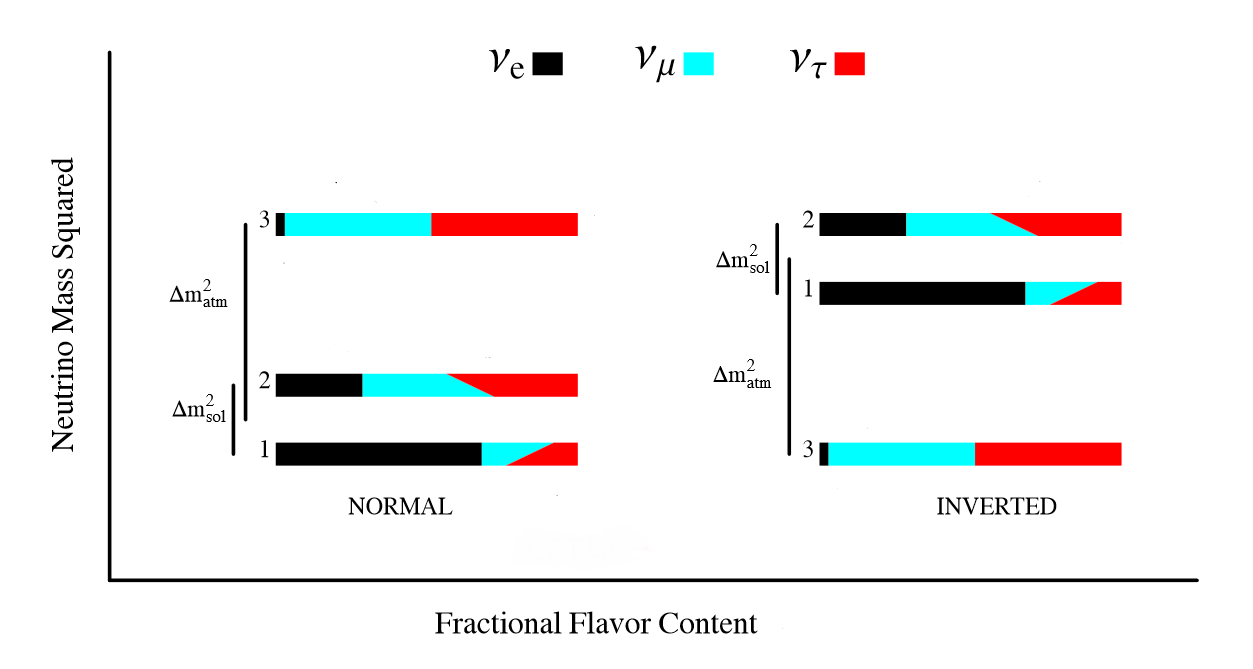
\includegraphics[scale=0.4]{neutrinos.png}
\captionof{figure}{The two hierarchies of neutrino mass states.  Black, teal, and red indicated the three flavors of neutrinos, while one, two, and three indicated the three mass states. Reproduced from Reference \cite{Parke}.}
\end{center}


The density parameter of neutrinos is given by
\[\Omega_\nu=\frac{\rho_\nu}{\rho_c}=\frac{1}{h^2}\sum_{i=1}^3 \frac{g_i m_i}{90eV},\]
where $g_i = 1$ for Majorana neutrinos (own antiparticle) and $g_i = 2$ for Dirac neutrinos (distinct antiparticles) \cite{Pastor}. Using the lower mass limit of the neutrino and assuming Majorana neutrinos, this suggests a lower limit on the neutrino density parameter of $\Omega_\nu \gtrsim 0.00122$.  Thus, neutrinos do provide some contribution to the nonbaryonic dark matter density parameter.  

To find an upper limit on the neutrino contribution to the nonbaryonic dark matter density parameter is is necessary to distinguish hot dark matter from cold dark matter.  Hot dark matter is composed of particles that have zero or nearly-zero mass.  Special relativity requires that the massless particles move at the speed of light, and that the nearly-massless particles move close to the speed of light.  As a result hot dark matter forms very hot gases.  Cold dark matter is composed of particles that have sufficient mass to travel at sub-relativistic velocities, thus forming colder gases.  With their low masses neutrinos fall under the hot dark matter category.  A combination of galaxy clustering measurements, CMB observations, and Lyman-$\alpha$ observations give an upper limit on the hot dark matter contribution of $\Omega_\nu \lesssim 0.0155$, thus neutrinos and other hot dark matter particles can not be the primary contribution to the nonbaryonic dark matter density parameter \cite{Spergel}.

If we assume cold dark matter (CDM) particles were in thermal equilibrium with the other standard-model particles during the early stages ($<$1 ns) of the universe it is possible to calculate the CDM density parameter.  According to Maxwell-Boltzmann statistics, as the temperature, $T$, of the universe cools, the particles with masses $m > T$ will diminish exponentially.  Once the temperature of the universe cooled below the CDM mass scale the creation of these particles would have ceased.  At this time the CDM particles which still existed would have continued annihilating with one another.  As time went on, CDM annihilation became less and less likely due to their dwindling abundance.  Once the expansion rate of the universe, given by Hubble's constant, exceeded the CDM annihilation/creation rate, the CDM particles dropped out of thermal equilibrium and the CDM density became fixed.  

The density parameter for CDM is approximately given by
\[\Omega_\chi h^2 \simeq \frac{T_0^3}{M_{Pl} \langle \sigma_A \nu \rangle} \]
where $\sigma_A$ is the total annihilation cross section of CDM particles, $\nu$ is the relative velocity of CDM particles, $T_0$ is the equilibrium temperature, $M_{Pl}$ is the Planck mass, $c$ is the speed of light, and $\langle ... \rangle$ represents an average over the thermal distribution of CDM particle velocities \cite{Kolb,Jungman}. Remarkably, for the total density parameter of the universe to equal unity, as required by cosmological models, a cross section on the order of particles interacting on the electroweak scale is required for CDM particles. This result is the main motivation behind suspecting weakly interacting massive particles (WIMPs) as the dominant contribution to the nonbaryonic dark matter density parameter.  These WIMPs are theorized to have a mass ranging from $\sim$ 10 GeV to a few TeV with an interaction cross sections on the order of the electroweak scale.  

\subsection{WIMPs and SUSY}

Supersymmetry (SUSY) is a symmetry of space-time which has been proposed in an effort to unify the electroweak, strong, and gravitional forces.  This theory offers some insight into the nature of WIMPs.  SUSY requires that a supersymmetric partner particle exist for each particle in the standard model.  These partners go by the names of sleptons (partners of leptons), squarks (partners of quarks), gauginos (partners of gauge bosons), and higgsinos (partners of Higgs bosons).  Sleptons and squarks have spin zero, while gauginos and higgsinos have spin one-half.  Since none of these supersymmetric particles have been discovered it is thought they are far more massive than their standard model counterparts, and thus that supersymmetry is not an explicit symmetry of nature.
  
Goldberg \cite{Goldberg} and Ellis \cite{Ellis} have suggested that neutral gauginos and neutral higgsinos can mix together in a superposition known as the neutralino, $\chi$.  In most SUSY models, the neutralino is the lightest supersymmetric particle (LSP).  In models which conserve R-parity (a new quantum number distinguishing SUSY particles from standard model particles) the LSP is stable, making it a prime candidate particle for dark matter.  The expected cross section of neutralinos interacting via inelastic collisions with nucleons is dependent on the allowed regions of parameter space in the SUSY model being used.  Results from the WMAP satellite refined this parameter space, concluding that the density parameter of neutralinos would be  $0.192 < \Omega_\chi < 0.263$ \cite{Spergel,Bennett,Arnowitt}.

\subsection{Other Dark Matter Candidates}

The neutralino is one of many candidate particles suggested for WIMPs, and as previously mentioned, WIMPs are not the only candidate for dark matter.  In this section we will briefly discuss some of the other candidates, as shown in Figure 3.

\begin{center}
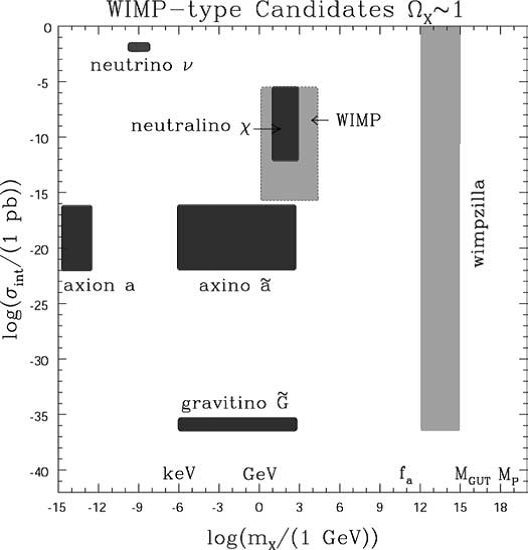
\includegraphics[scale=0.7]{DMCandidates.png}
\captionof{figure}{Estimated interaction strengths ($\sigma_{int}$) of some of the dark matter candidates with masses $m_\chi$. Reproduced from Reference \cite{Roszkowski}.}
\end{center}

\subsubsection{Axions and Axinos}
Quantumn chromodynamics (QCD) is a theory describing the strong interaction between quarks and gluons, which make up hadrons.  In particle physics there exists a proposed symmetry of nature referred to as charge conjugation parity symmetry (CP-Symmetry).  CP-Symmetry postulates that particles should behave the same if they are replace by their own antiparticle (C symmetry), and then have their parity reversed (P symmetry). Within QCD there is no theoretical reason to assume CP-symmetry exists.  However, when a CP-violation term is included in the QCD lagrangian its coefficient has been experimentally determined to be less than $10^{-10}$ \cite{Baluni}. This unexpected result is known as the strong CP problem in quantum chromodynamics.    To reconcile this, a new symmetry known as the Peccei-Quinn theory has been proposed.  This theory postulates the existence of a new pseudoscalar particle called the axion.  According to the Peccei-Quinn theory, axions would be electrically neutral, low mass ( $1\mu eV - 1 eV$) particles which have very low interaction cross-sections for the strong and weak forces.  The axino arises when SUSY is introduced to the Peccei-Quinn theory, resulting in a supersymmetric partner to the axion known as the axino.

\subsubsection{Gravitons and Gravitinos}
In quantum field theory, the graviton is a hypothetical  elementary particle which mediates the gravitational force.  As with axions and axinos, when SUSY is introduced to quantum field theory a supersymmetric partner to the graviton is predicted to exist known as the gravitino.  In some models, gravitinos are the LSP in SUSY and are thus a candidate particle for dark matter.

\subsubsection{WIMPzillas}
The final dark matter candidate shown in Figure 3 is the WIMPzilla.  WIMPzillas are supermassive dark matter particles which arise when one considers the possibility that dark matter might be composed of nonthermal supermassive states. These particles would have a mass many order of magnitude higher than the weak scale \cite{Chung}. Studies have shown that for stable particles with masses close to $10^{13} \; GeV$  WIMPzillas would be produced in sufficient abundance to give $\Omega \approx 1$ for the total density parameter of the universe.  

It should be noted that Figure 3 and the discussion of this section does not encompass all of the alternatives to WIMPs.   Although these other dark matter candidates offer intriguing explanations to the dark matter problem, we will now discuss WIMPs and direct WIMP detection experiments.


\section{Direct Detection of WIMPs}

\subsection{WIMP Recoil Spectrum}
Cold dark matter particles such as WIMPs can be detected directly via nuclear recoils in terrestrial detectors.  In these events, a WIMP will scatter off of a target nucleus in the detector, causing the nucleus to recoil with a certain amount of energy taken from the collision.  The expected energy recoil spectrum of WIMPs detected in this manner is given by
\[\frac{dN}{dE_r}=\frac{\sigma_0 \rho_\chi}{2 \mu^2 m_\chi} F^2(q) \int_{v_{min}}^{v_{esc}} \frac{f(v)}{v} dv, \]
where $\rho_\chi$ is the local WIMP density, $f(v)$ is the velocity distribution of WIMPs in the halo, $v_{min}$ is the minimum WIMP velocity able to generate a recoil of energy $E_r$, $v_{esc}$ is the escape velocity for WIMPs in the halo, and  $\sigma_0$ is the WIMP-nucleus interaction cross sections. $F(q)$ is the nuclear form factor describing the scattering amplitude for momentum transfer $q$,and $\mu$ is the WIMP-nucleus reduced mass given by 
\[\mu=\frac{m_\chi m_N}{m_\chi + m_N}\]
where $m_N$ is the target nucleus mass \cite{Jungman,Goodman,Lewin}. The WIMP-nucleus cross section can have both spin-independent (SI) and spin-dependent (SD) components \cite{Shan}. The SI interaction cross section is given by
\[\sigma_0^{SI}=\frac{4}{\pi}\mu^2 [Z f_p + (A - Z) f_n]^2,\]
where Z is the atomic number of the target nucleus (the number of protons), A is the atomic mass number of the target nucleus ($A-Z$ is therefore the number of neutrons in the nucleus), and $f_p$ and $f_n$ are the effective scalar couplings of WIMPs to protons and neutrons, respectively.  In this process we must sum over the interactions in each nucleon prior to squaring, since the DeBroglie wavelength associated with the momentum transfer is comparable to, or larger than, the size of the target nuclei, giving rise to a coherence effect across the nucleons.  If the scalar couplings of WIMPs with neutrons and protons are approximately equal (which is the case with the LSP of SUSY), then the SI cross section can be simplified to
\[\sigma_0^{SI} \simeq \frac{4}{\pi}\mu^2 A^2 |f_p|^2. \]
The cross section for SD interactions is given by
\[\sigma_0^{SD}=\frac{32}{\pi}G_F^2\mu^2\frac{J+1}{J}[\langle S_p \rangle a_p + \langle S_n \rangle a_n]^2, \]
where $G_F$ is the Fermi constant, $J$ is the total spin of the target nucleus, $\langle S_{(p,n)} \rangle$ are the expectation values of the proton and neutron group spins, and $a_{(p,n)}$ are the effective SD WIMP couplings on protons and neutrons.  In SD WIMP-nucleus interactions it is assumed that only unpaired nucleons contribute significantly to the total cross section, since the spins of the nucleons in a nucleus are anti-aligned.  In most cases, the spin independent, coherent term dominates the total WIMP-nucleus cross section due to its $A^2$ dependence on the atomic mass number of the target nucleus.

A calculation of both the differential and integrated WIMP event rates in single isotope targets of  $^{131}$Xe, $^{73}$Ge, and $^{40}$Ar using a WIMP mass of 100 GeV is included in Figure 4.

\begin{center}
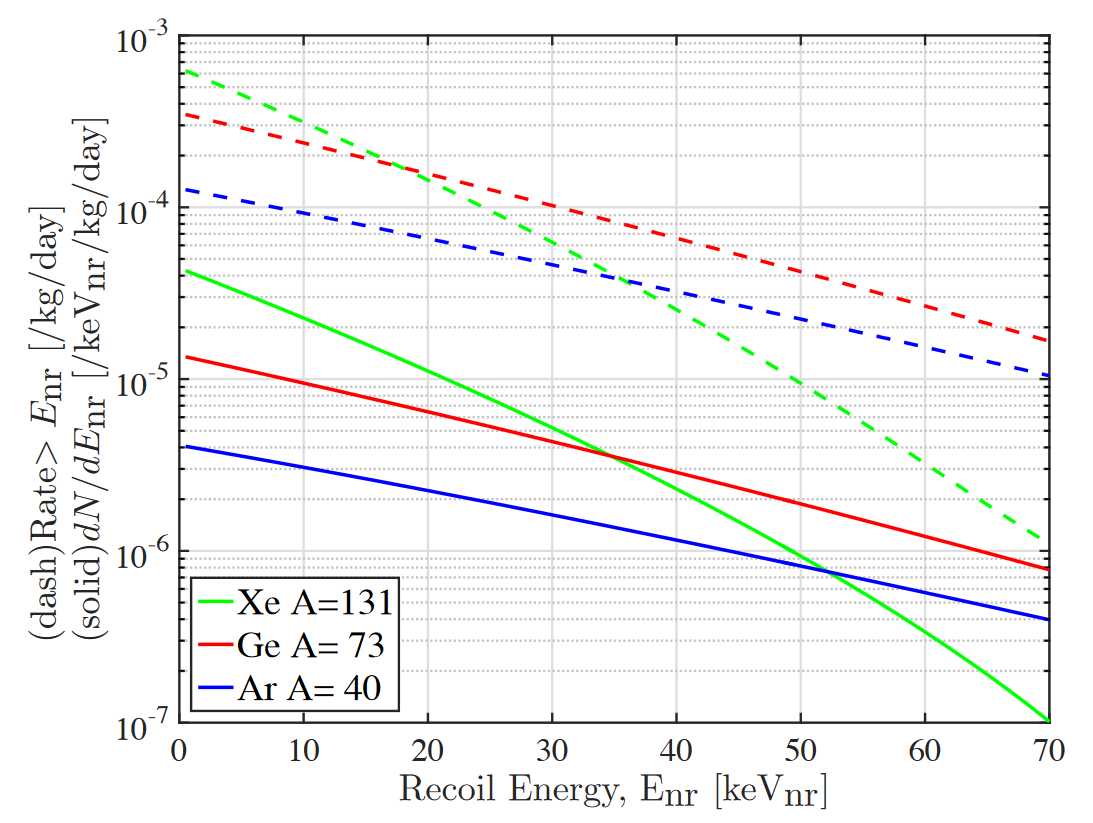
\includegraphics[scale=0.5]{Recoil-spectrum.png}
\captionof{figure}{Calculated differential spectrum in evts/keV/kg/d (solid lines) and the integrated event rate in evts/kg/d (dashed lines)  for $^{131}$Xe, $^{73}$Ge, and $^{40}$Ar assuming a 100 GeV WIMP with spin-indepdent cross section for a WIMP-nucleon of $\sigma=5 \times 10^{-43} cm^2$.}  
\end{center}

Lighter target nuclei will produce lower event rates in a WIMP detector due to their lower cross sections (resulting from lower $A^2$ contribution in the coherent SI term) and less effective transfer of energy during nuclear recoil events. While heavier target nuclei produce stronger interaction cross sections, they also result in reduced event rates at high energies due to a loss of coherence from form factor suppression.  To maximize efficiency a xenon detector with a low analysis threshold is ideal.

\subsection{Quenching Factors and Event Discrimination}
In WIMP detectors there will be two types of events.  WIMPs and neutrons will deposit energy via nuclear recoils, while gamma rays and x-rays will deposit energy via electron recoils.  The key to identifying WIMP events within a detector lies in understanding how it will respond to each of these events.  To achieve this goal, a quantity known as the quenching factor of a detector must be determined.  The quenching factor of a detector describes the difference in the amount of energy measured by the detector between the two types of events.  Electron recoil events are typically measured in units of $keV_{ee}$ ("keV-electron-equivalent"), which is the amount of energy an electron recoil would require to generate the event.  Similarly, nuclear recoil events are typically measured in units of $keV_{nr}$ ("keV-nuclear-recoil"), which is the amount of energy a nuclear recoil would require to generate the event.  The energy scale for electron recoils can be set using a beta emitting calibration source, while the energy scale for nuclear recoils can be set using a neutron calibration source.  A detector's quenching factor is then given by
\[QF=\frac{E_{ee}(keV_{ee})}{E_r(keV_{nr})}.\]

In two phase (liquid and gas) xenon detectors the quenching factor differs between scintillation and ionization signals produced by interactions within the liquid.  The initial recoil event will produce a scintillation signal (referred to as S1) and ionization.  Photo-multiplier tubes can be used to measure the scintillation light, while the ionization can be drifted to an anode located in the gas phase of the detector.  Once the charged particles are accelerating toward the anode in the xenon gas they will create a secondary scintillation signal (referred to as S2).  Nuclear recoil events have higher ionization density, leading to a higher recombination probability, resulting in a higher S1 yield and lower S2 yield than electron recoil events of the same energy. Thus, the different quenching factors can be used to distinguish the two types of events.

\begin{center}
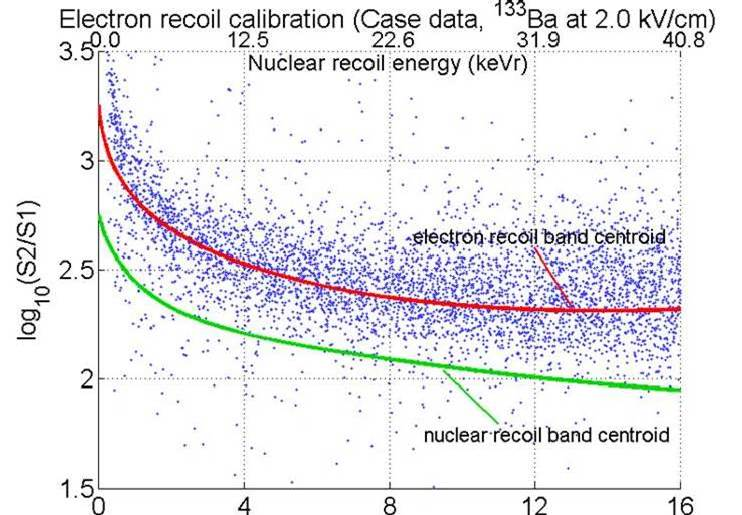
\includegraphics[scale=0.75]{Recoils.jpg}
\captionof{figure}{A plot of electron recoil events generated by an external calibration source in the LUX prototype (LUX 0.1).  This data is used to determine the electron recoil band shown in red, while data from a neutron source (not shown) is used to determine the nuclear recoil band shown in green }
\end{center}

\section{The Large Underground Xenon Detector}

\subsection{Introduction to LUX}
The Large Underground Xenon detector (LUX) is a dual phase time projection chamber containing 350 kg of xenon used as the target mass for WIMP detection. (Figure 6) The xenon is cooled by a thermosyphon system until it condenses in the detector.  Inside of the xenon space there is one photo-multiplier tube array submerged in the liquid xenon, another photo-multiplier tube array suspended in the xenon gas, and five wire grids producing an electric field to drift charged particles through the detector.  The location of the S2 signal provides the x and y coordinates of the recoil event, while the time between the S1 and S2 signal provides the z coordinate of the recoil event.  This allows the primary event to be localized within one centimeter in all three spacial dimensions.  The xenon space is shielded by a 300 ton water tank which houses additional photo-multiplier tubes for cosmic ray vetoing \cite{McKinsey,Fiorucci}.

\begin{center}
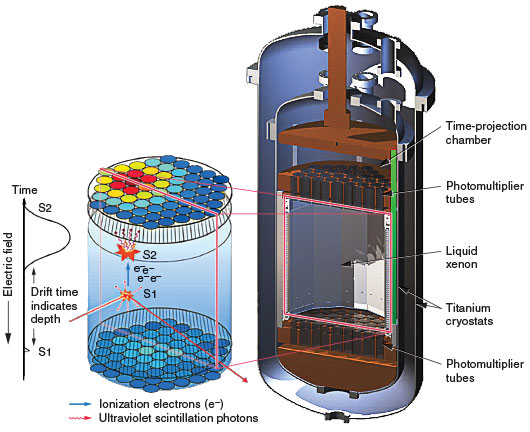
\includegraphics[scale=0.5]{lux.jpg}
\captionof{figure}{Image depicting the internals of the LUX detector.}
\end{center}

\subsection{Calibration of the Detector}

In order to distinguish dark matter signals in the detector from background signals the detector's response to nuclear recoil events and electron recoil events must be well understood. (Figure 5) For calibrating electron recoil events it is common to use an external beta emitter such as cesium-137.  However, the xenon in LUX has a strong self-shielding characteristic at UV wavelengths.  While this is convenient for eliminating background radiation, it makes calibrating the inner most regions of a detector the size of LUX a challenge.

To overcome this problem LUX is making use of internal calibration sources.  An ideal internal calibration source would need to be a single beta emitter in the energy range of interest ($ <15 $ keV) which can be dissolved into the liquid xenon in the detector.  Furthermore, the source must be made of a material with low electronegativity so that it will not poison the detector's charge drift length.  Similarly the source can not attenuate the UV scintillation light produced by events in the detector.  To achieve a reliable calibration in all regions of the detector the source would need to have a long enough life time to diffuse throughout the entire detector (a few hours).  Finally, there must be a method for removing the source once the calibration has finished.  This could simply mean waiting for the source to decay if its half life is short, or actively purifying the source out of the detector if its half life is long \cite{Kastens}.

Tritium meets several of these requirements.  It is a beta emitter with a Q-value of 18 keV that produces a broad spectrum over the entire energy range of interest.  Its 12.3 year half life means that the source will have plenty of time to dissolve uniformly throughout the detector.  However, this long half life is potentially dangerous, since one can not simply wait for it to decay away -- it must be actively removed from the detector when the calibration is completed.  To complicate this matter bare tritium sticks to most surfaces, including materials like teflon, polyethylene, and steel which make up the majority of most xenon detectors.

To make tritium removal more feasible we have made use of tritiated methane (CH$_3$T).  Methane is highly inert due to its fully saturated carbon-hydrogen bonds.  It has a diffusion constant in polyethylene that is 10 times smaller than hydrogen, and it does not capture electrons that will be drifting through the detector.  By replacing one of the hydrogen atoms in a methane molecule with tritium we combine the strength of both of these materials, resulting in the ideal internal calibration source.


\subsection{Gas Experiments}

To study CH$_3$T removal we built a system to inject tritiated methane into a gaseous xenon environment.  This system consists of three sections. 

\begin{center}
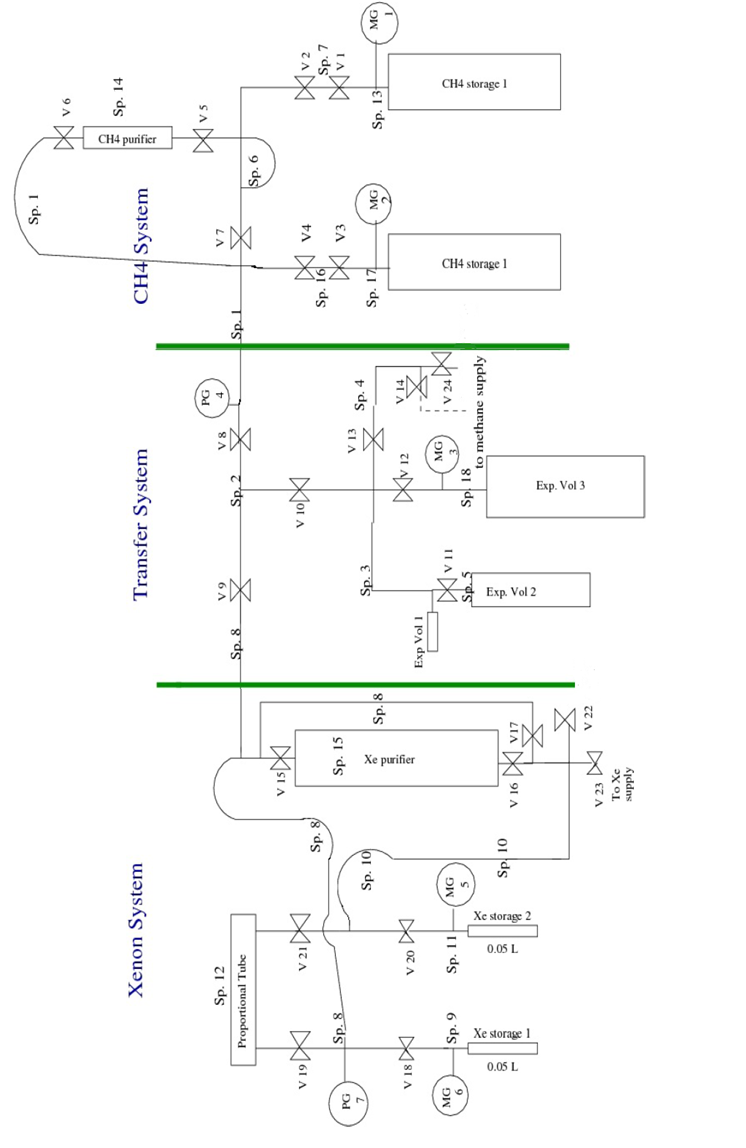
\includegraphics[scale=0.5]{GasSystem.png}
\captionof{figure}{CH$_3$T gas system at UMD.  Three sections of the system are distinguished with green lines. Circles labeled PG and MG are pressure gauges, and the hourglass shapes represent hand valves.}
\end{center}

The first section, the xenon space, contains a xenon purifier which uses hot zirconium to remove the CH$_3$T, two xenon storage bottles used to move xenon through the system via cryopumping, and a proportional tube used to detect activity within the xenon space.  The second section is a small transfer system which is used to inject consistent amounts of CH$_3$T into the xenon space with each injection.  The final section consists of a CH$_3$T storage bottle used as the source of injections and a SAES MC1-905F methane purifier to remove unwanted contaminates prior to entering the xenon space.

The primary goal of this experiment was to determine the purification efficiency and study residual contamination.  There are two factors which dominate purification efficiency -- flow rate through the purifier and rest time between subsequent purifications.  High flow rates through the purifier can cool the zirconium inside, while inadequate rest time between purifications can lead to build up of methane on the surface of the zirconium beads.  Both of these situations lead to a decrease in purifier efficiency. 

The first black data point in Figure 8 is our worst purification efficiency, (96\% +/- 1\%) corresponding to our highest flow rate. (8 SLPM compared to the typical ~0.3 SLPM)  While we were unable to control the flow through our experiment as much as we desired, we are at least able to conclude that exceeding the maximum flow rate suggested for the purifier does significantly decrease purification efficiency.

\begin{center}
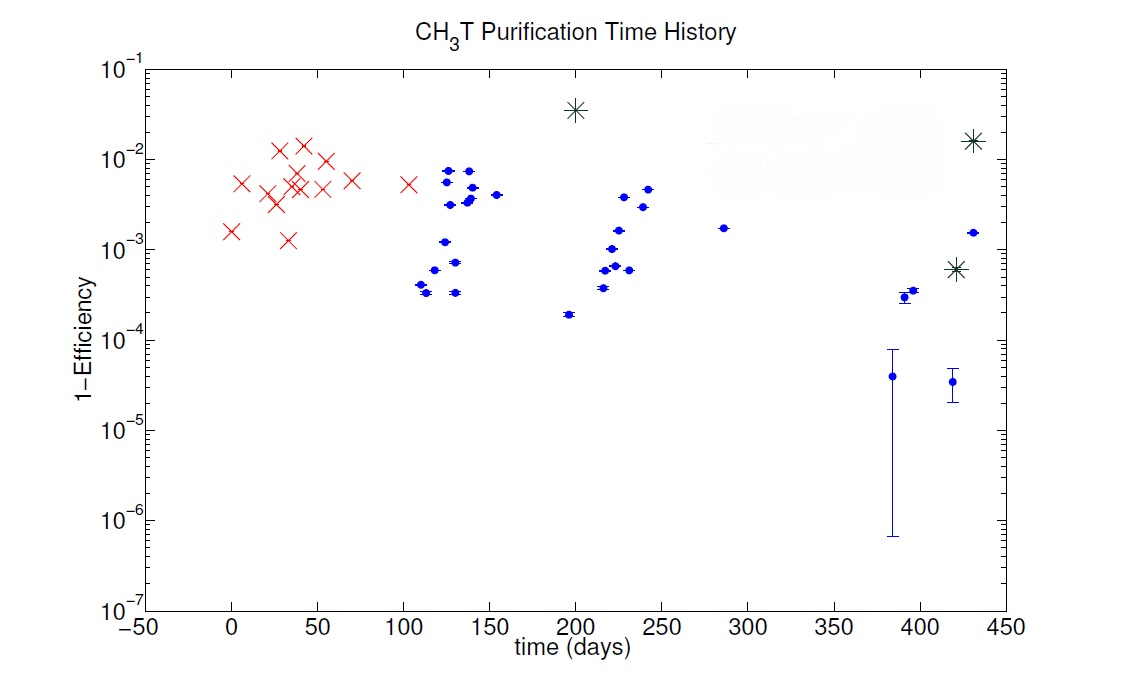
\includegraphics[scale=0.5]{Figone.jpg}
\captionof{figure}{Single pass inefficiency of the purifier when removing CH$_3$T.  The red and blue points indicate data taken by different students, while the black points indicate data for which the procedures were intentionally altered. }
\end{center}

We found that allowing for ample rest time between purifications does significantly increase purification efficiency. Our best purifications were the first data points in each cluster in Figure 9.  We were able to obtain efficiencies of 99.99\% when the purifier was resting for three weeks or longer, and obtained efficiencies of 99\% to 99.9\% when the purifier was used on a daily basis.

\begin{center}
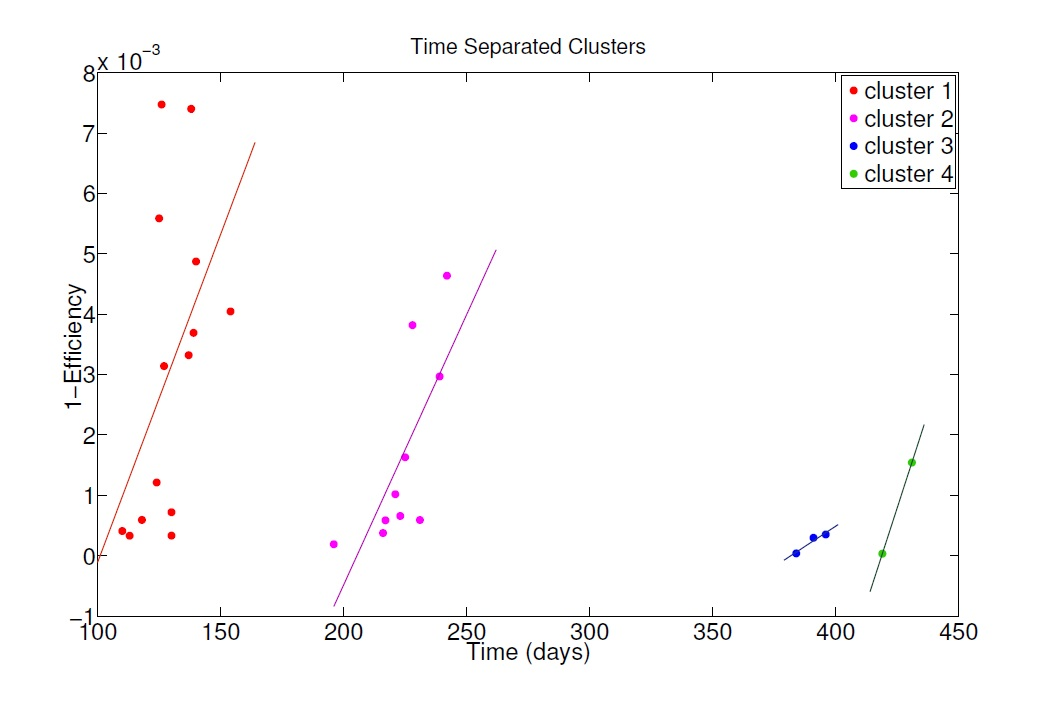
\includegraphics[scale=0.5]{Figfour.jpg}
\captionof{figure}{Time-separated clusters of purifications have an upward trend in purification inefficiency.  Each cluster shown is separated in time by at least three weeks.}
\end{center}

\subsection{Liquid Experiments}

We have also tested tritium removal from liquid xenon.  Our liquid xenon system consists of two main sections, the CH$_3$T injection system and the liquid xenon system.  We will first discuss the set up of the tritium injection system, pictured below.

\begin{center}
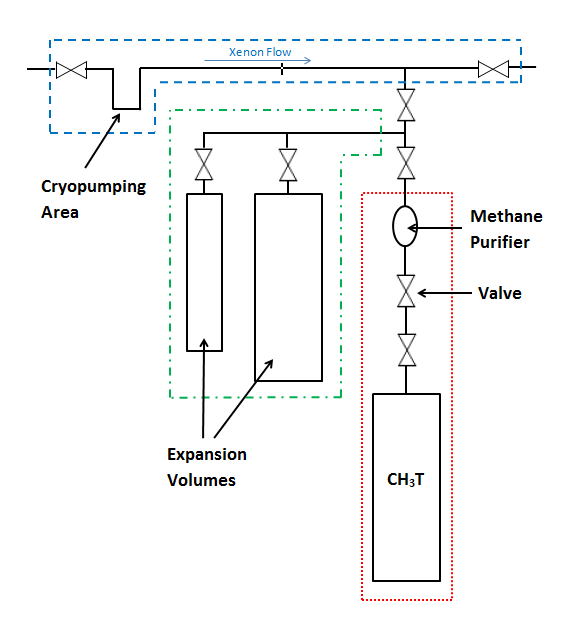
\includegraphics[scale=0.8]{UMDInjectionSys.png}
\captionof{figure}{The tritium injection system for the liquid phase experiments at UMD. The red box indicates the CH$_3$T storage bottle and methane purifier area, the green box indicated the expansion volumes, and the box indicates the cryopumping and xenon flow through area.}
\end{center}

The injection system begins at the CH$_3$T storage bottle.  This bottle is double valved for safety reasons.  As with the gaseous experiments, we have a SAES MC1-905F methane purifier in series with the storage bottle.  Following the methane purifier there is a series of injection volumes branching off to the left.  These injection volumes are designed to inject the desired amount of CH$_3$T into the xenon system.  The last component of the injection system is located above the injection volumes.  This plumbing is used to collect all of the CH$_3$T from the injection volume via cyropumping.  After the plumbing has warmed, the xenon circulating outside of the injection system is rerouted through the cryopump plumbing to sweep all of the CH$_3$T into the xenon system.

The second section of our system, the liquid xenon system, is pictured below.

\begin{center}
\includegraphics[scale=0.75]{cryo.png}
\captionof{figure}{The liquid xenon system at UMD. (A) The xenon condenser consists of a helical coil cooled by a pulse tube refrigerator.  (B) The liquid xenon storage vessel houses two PMTs to observe tritium decay.}
\end{center}

In the liquid xenon system, a pulse tube refrigerator cools a xenon gas condenser consisting of a helical coil of copper tubing.  The condensed xenon then drips into a liquid xenon storage vessel.  Inside of the liquid xenon storage vessel are two PMTs that face each other. These PMTs are used to observe xenon scintillation light from tritium decay. Once the vessel is filled both of these PMTs are submerged in the liquid xenon.  Note that this means the system at UMD is a single phase detector, rather than a dual phase detector like LUX.  Polyethylene or teflon curtains were installed in the inner cryostat to surround the PMTs during some of our data sets.  These curtains of plastic were used to study out gassing effects in our detector.  It should be noted that in the plumbing leading to the liquid xenon system there is a SAES Zirconium getter (pcf4c3r1) used to purify the tritiated methane out of the system when desired.

During our liquid phase experiments, our experimental procedure consisted of taking an adequate amount of background data, injecting CH$_3$T into the liquid xenon, waiting for the CH$_3$T event rate to plateau, then purifying the CH$_3$T out of the xenon.  During the data sets in which teflon or polyethylene curtains were installed around our PMTs we bypassed our purifier after initally purifying away the CH$_3$T so that out gassing effects could be studied.  Injection activities for our liquid phase experiment ranged from 1487 $\pm$ 35.06 Bq to 12164 $\pm$ 1028.11 Bq.  

A detailed list of our purification efficiency in liquid xenon is included in Table 1.  Note that the rise in background rate during our polyethylene runs is due to a change in PMT gain.  Using the lessons learned from the gaseous xenon experiments we were able to achieve an average purification efficiency of 99.999\% in our liquid experiments, where we define our purification efficiency to be

\begin{center}
Purification Efficiency $= 1 - \frac{A - B}{I - B},$
\end{center}

\noindent
where $A$ is the background event rate after injecting CH$_3$T, $B$ is the background event rate prior to injecting CH$_3$T, and $I$ is the injected CH$_3$T activity as observed by out PMTs.  We find that the addition of plastic curtains around our PMTs does not impair our ability to remove CH$_3$T at $>$ 99.998\% levels.  To illustrate the effectiveness of CH$_3$T removal, an overlay of injected and purified CH$_3$T spectra is included in Figure 12.  

\begin{center}
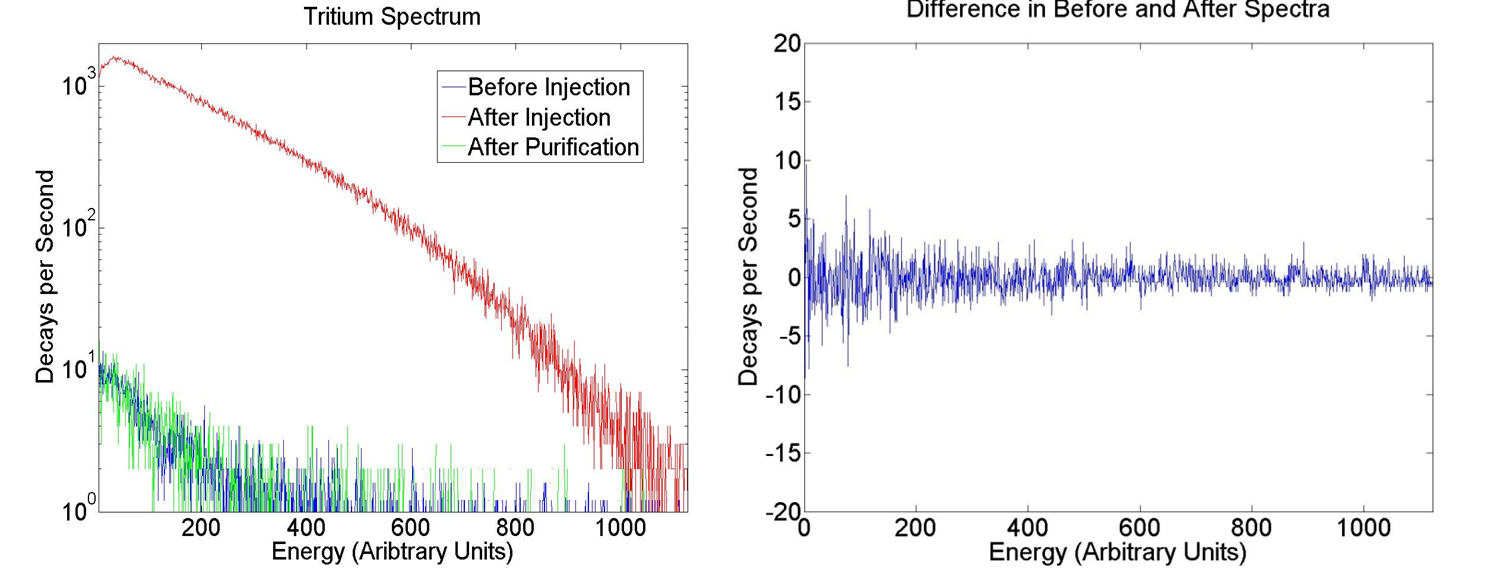
\includegraphics[scale=0.5]{spectra.png}
\captionof{figure}{Left: Overlay of spectra seen by PMTs in the liquid xenon detector.  The blue spectrum is what is seen by the PMTs prior to injecting tritium, the red spectrum is what is seen by the PMTs after injecting tritium, and the green spectrum is what is seen by the PMTs after purifying the xenon to remove any injected tritiated methane.  Right: The difference between the before injection and after purification spectra. }
\end{center}

\begin{sidewaystable}
\scalebox{0.9}{
\centering
\caption{CH$_3$T purification efficiencies in liquid xenon.}
\begin{tabular}{ c | c | c | c | c }
Observed Injection Activity (Bq) & Background Before Injection (Bq) & Background After Injection (Bq) & Purification Efficiency & Type of Plastic \\
\hline
10415.84 $\pm$ 140.89 & 4.78 $\pm$ 0.38 & 4.99 $\pm$ 0.39 & 0.99998 $\pm$ 0.000054 & No Plastic \\
3295.15 $\pm$ 46.28 & 4.99 $\pm$ 0.39 & 5.01 $\pm$ 0.39 & 0.99999 $\pm$ 0.00017 & No Plastic \\
2836.67 $\pm$ 22.35 & 5.01 $\pm$ 0.39 & 4.76 $\pm$ 0.39 & 1.00009 $\pm$ 0.00020 & No Plastic \\
12164.29 $\pm$ 1028.11 & 4.72 $\pm$ 0.39 & 5.09 $\pm$ 0.39 & 0.99997 $\pm$ 0.000082 & No Plastic \\
11033.62 $\pm$ 1766.87 & 5.09 $\pm$ 0.39 & 4.69 $\pm$ 0.38 & 1.00004 $\pm$ 0.00015 & No Plastic \\
9435.13 $\pm$ 180.13 & 3.74 $\pm$ 0.38 & 5.32 $\pm$ 0.39 & 0.99983 $\pm$ 0.000061 & Teflon \\
7666.08 $\pm$ 226.67 & 5.11 $\pm$ 0.39 & 5.23 $\pm$ 0.39 & 0.99998 $\pm$ 0.000082 & Teflon \\
6043.72 $\pm$ 446.80 & 5.23 $\pm$ 0.39 & 5.23 $\pm$ 0.39 & 1.00000 $\pm$ 0.00016 & Teflon \\
4504.81 $\pm$ 220.89 & 4.64 $\pm$ 0.39 & 4.71 $\pm$ 0.40 & 0.99998 $\pm$ 0.00016 & No Plastic \\
1487.09 $\pm$ 35.06 & 5.79 $\pm$ 0.41 & 5.76 $\pm$ 0.41 & 1.00002 $\pm$ 0.00043 & Polyethylene \\
\end{tabular}
}
\end{sidewaystable}


Cumulatively, we have injected over 68,000 becquerel of CH$_3$T into our liquid xenon.  Although systematic errors lead to a fluctuation of our residual background rates, we see no upward trend in our data set as the cumulative observed injection activity rises.(Figure 13)


\begin{center}
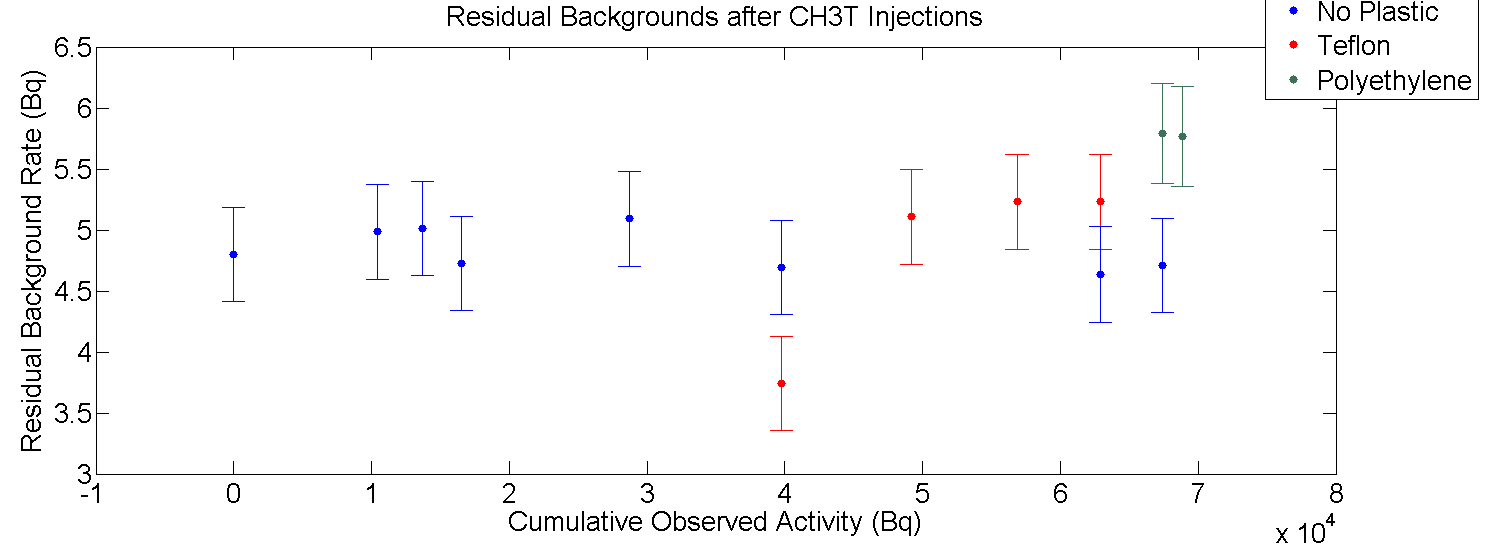
\includegraphics[scale=0.3]{ResidualBackgroundCorrected_SystemErr.png}
\captionof{figure}{Residual background rates over time in our detector after purifying the CH$_3$T out of the xenon. Blue data points are data sets in which no plastic curtains where used inside of the detector, red data points are data sets in which teflon curtains where used inside of the detector, and green data points are data sets in which polyethylene curtains were used inside of the detector.}
\end{center}

\subsection{Out Gassing Experiments}

To more accurately model the LUX detector we surrounded our PMTs with polyethylene or teflon panels during some of our data sets.  The experimental procedure for these data sets was to collect an adequate amount of background data, inject CH$_3$T into the liquid xenon, wait for the CH$_3$T event rate to plateau, purify the CH$_3$T away until we reached the initial background event rate, then bypass the purifier on our system to study out gassing effects.  Once the purifier had been bypassed we discovered two sources of residual CH$_3$T contamination.  

\begin{center}
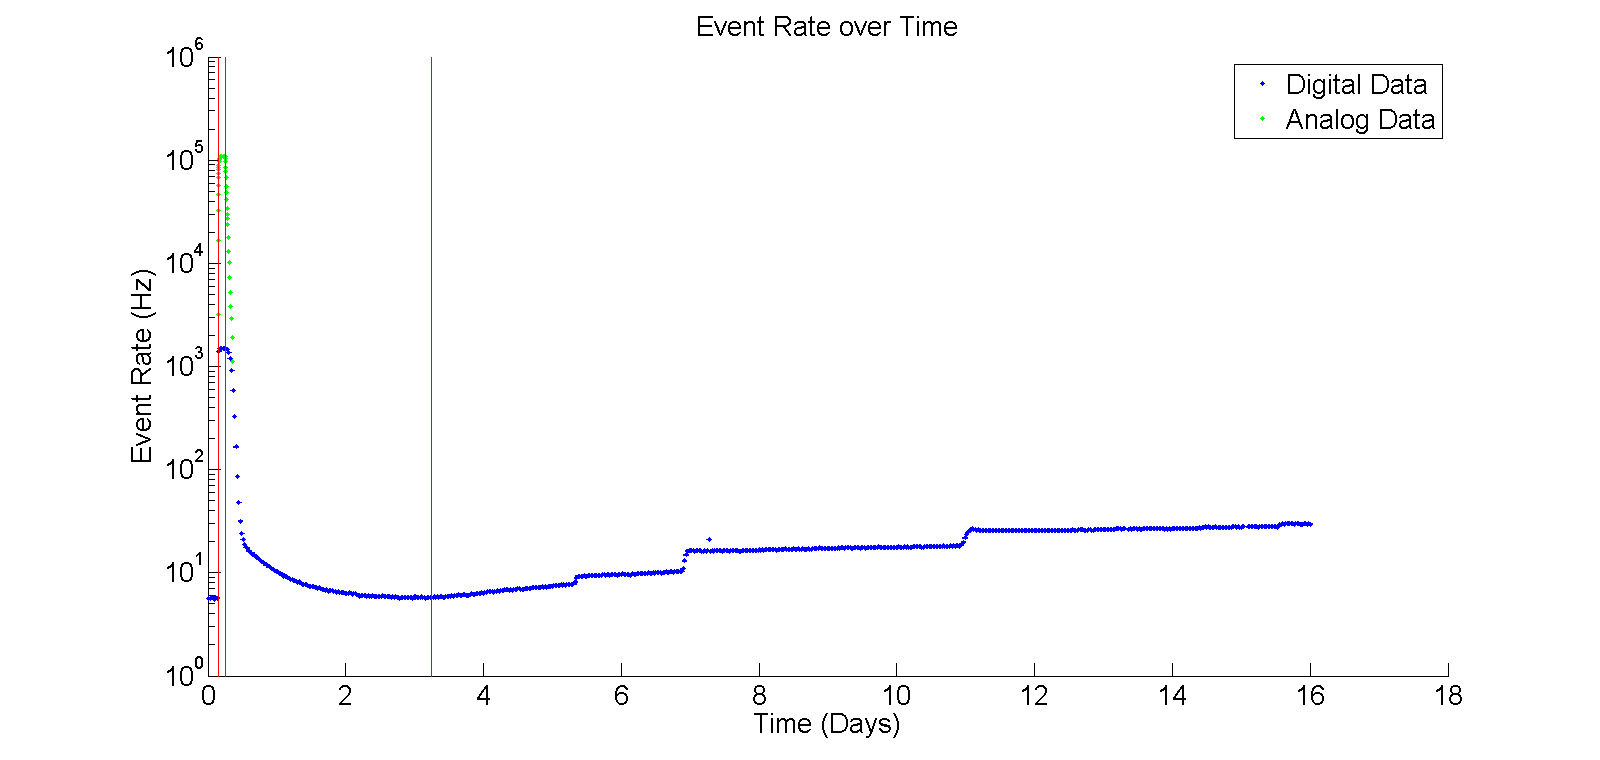
\includegraphics[scale=0.4]{Outgassing_TimeHisto_Log.png}
\captionof{figure}{A continuation of the time histogram shown in Figure 14.  The third red line indicates when our purifier was bypassed. A gradual rise in CH$_3$T activity is apparent after bypassing the purifier, accompanied with occasional large leaps in CH$_3$T activity.}
\end{center}

We see a gradual rise in CH$_3$T activity after bypassing our purifier due to out gassing of CH$_3$T from the plastic panels.  This out gassing effect will be discussed in detail in Section 4. In addition to this steady rise, we see large steps in CH$_3$T activity at random intervals. (Figure 14)  These step features occur every ~3 days on average.  The longest period of time without a step occurring was 5.08 days. To examine these step features more closely, we analyzed the spectra from one of these events.  We found that the integral of the spectra rose from 8833 $\pm$ 93.98 to 17190 $\pm$ 131.11 during the event, a increase of 194.6\%. (Figure 15)  

\begin{center}
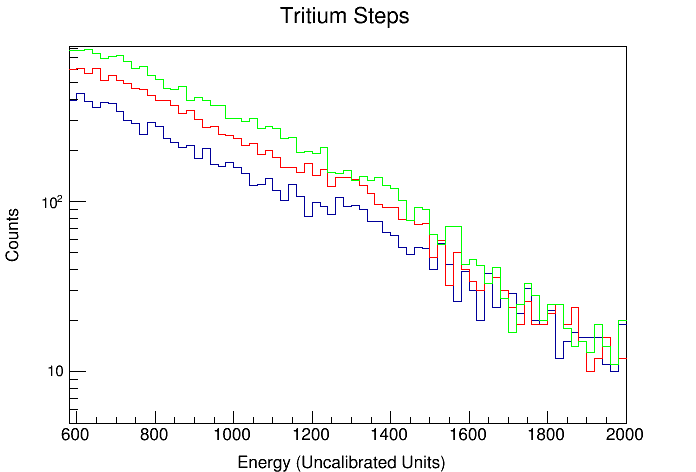
\includegraphics[scale=0.5]{Steps_Overlay.png}
\captionof{figure}{An overlay of three spectra from a step in CH$_3$T after bypassing our purifier.  The blue spectrum was collected prior to a step occurring, the red spectrum was collected while a step was occurring, and the green spectrum was collected after the step had reached a plateau.}
\end{center}

Such an increase in CH$_3$T activity can be produced through two mechanisms -- a drift in PMT gain which would shift the CH$_3$T spectrum horizontally, or an increase in CH$_3$T activity shifting the CH$_3$T spectrum vertically.  To determine if our PMT gain was shifting during our CH$_3$T data sets we used an external Cesium-137 to a construct time histogram of the Cesium-137 rate.  Over eight days the Cesium-137 event rate remained flat, with an initial event rate of 120255 $\pm$ 346.778 (observed Bq) and a final event rate of 115469 $\pm$ 339.807 (observed Bq).  A linear fit to the Cs-137 data results in a nearly zero slope of 0.0026 Bq per day.  (Figure 16) We conclude that the rise in tritium rate during the step events can not be due to our PMT gain drifting, and must therefore be a result of an increase in the amount of CH$_3$T in the fiducial region of our detector.  We suspect this increase in CH$_3$T is due to pockets of stagnant gas slowly moving into the detector's fiducial region.  To avoid such a source of residual CH$_3$T contamination, a detector wishing to using tritated methane as an internal calibration source must be designed such that no areas of stagnant gas exist within its system.

\begin{center}
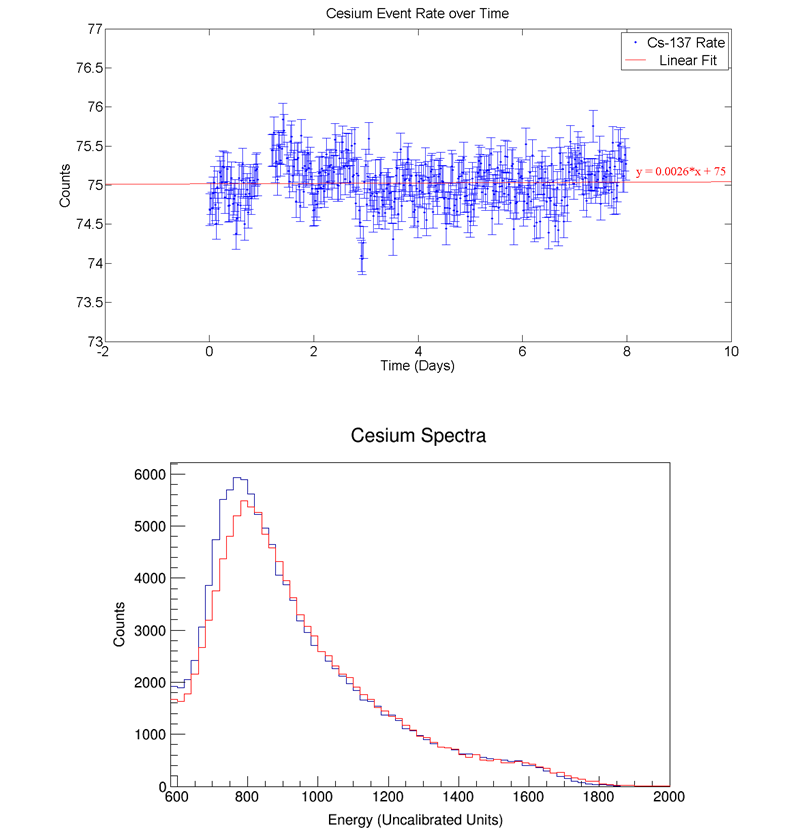
\includegraphics[scale=0.6]{Cesium_Combined_Fit.png}
\captionof{figure}{Top: A time histogram of Cesium-137 events in our detector. Bottom: An overlay of the initial Cs-137 spectrum and the final Cs-137 spectrum in the time histogram above.}
\end{center}

\section{Modeling Diffusion in LUX}

For an internal calibration of the LUX detector to be successful two conditions must be met.  First, there must be enough events detected during the calibration to accurately measure the tritium spectrum.  We choose to define a factor of 100 over the number of  background events which LUX collects over 300 days to be a sufficient number of CH$_3$T decays for the calibration.  The nominal background rate of LUX is $8.4 \times 10^{-4} \frac{events}{keV*kg*day}$.  Since the fiducial volume of LUX is 100 kg, and the energy spectrum of interest ranges from 1.3 keV to 8 keV, we expect 170 background events in LUX over 300 days.  Thus, we wish to collect around 17,000 events during our CH$_3$T calibration.  The second condition for a successful CH$_3$T calibration is that any residual CH$_3$T remaining after purification must not add a significant contribution to the background rate in the detector.  We choose to define the tolerable CH$_3$T activity after a calibration to be 5\% of the nominal background rate in LUX, setting a limit on the residual CH$_3$T activity of $8.4 \times 10^{-4} \frac{events}{keV*kg*day} \times 100 \; kg \times 6.7 \; keV \times \frac{1 \; day}{86400 \; sec} \times 0.05 = 0.33 \mu Bq$.

To achieve these goals we must determine how much initial CH$_3$T activity to inject into LUX by numerically modeling the purification and residual diffusion of CH$_3$T in LUX.  Fick's two laws are simple differential equations which describe the diffusion process.  The first law describes the flux of a material through a surface.  Its general form is given by
\[J=-D \nabla \phi,\]
where $J$ is the amount of material per unit area per unit time, $D$ is the diffusion coefficient, and $\phi$ is the concentration function of the material. Combining this with the continuity equation,
\[\frac{\delta\phi}{\delta t} + \nabla \cdot J =0,\]
which states that a change in density in any part of the system is due to inflow and outflow of material results in Fick's second law,
\[\frac{\delta \phi}{\delta t} = D \nabla^2\phi,\]
which describes the transport of a material by diffusion.

To implement these diffusion laws into our model we must determine the diffusion coefficient of CH$_3$T in the plastics of LUX.  At room temperature, the diffusion coefficient of methane in Teflon is measured to be $2.3 \times 10^{-7} \frac{cm^2}{sec} $. \cite{Miyake}  The temperature dependence of this diffusion constant is modeled by the Arrhenius equation,
\[D=Ae^{\frac{-E_a}{RT}},\]
where $E_a$ is the activation energy, $R$ is the gas constant, and $T$ is the temperature.  This suggests an adjustment factor to the diffusion constant of $10^{-6}$ at liquid xenon temperature.  This adjustment factor is equivalent to increasing the thickness of the plastic in our model by a factor of 1,000.  For this reason we are motivated to use half-infinite line boundary conditions in our diffusion model.

The analytic solution to Fick's second law using half-infite line boundary conditions is
\[\phi (x,t) = KC_{out} - \int \limits_0^t erf(\frac{x}{\sqrt{4D(t - \tau)}})K\dot{C_{out}}(\tau)d\tau - KC_{out}(0)erf(\frac{x}{\sqrt{4Dt}}),\]
where $K$ is the solubility of the material and $C_{out}$ is the outside concentration of the material. \cite{Piche} For the out gassing process we are only interested in the flux of material out of the plastic.  This is given by Fick's first law evaluated at $x=0$,
\[J_{out}(t)= - K \sqrt{\frac{D}{\pi}}( \int \limits_0^t \frac{\dot{C_{out}}(\tau)}{\sqrt{t-\tau}} d \tau + \frac{C_{out}(t)}{\sqrt{t}}),\]
where the sign has been flipped since the flux of material is outward.  We see that it is no longer possible to evaluate $K$ and $D$ separately, since the diffusion in and out of the plastic is completely determined by the time-dependent concentration outside of the plastic.  To simplify our model, we define a new constant
\[ G = K \sqrt{ \frac{D}{ \pi }} .\]

We can fit the integral of our equation for the flux out of the plastic over time to the out gassing data collected in Maryland's liquid xenon system to extract a value for the constant $G$. Since this out gassing data includes step features from stagnant pockets of unpurified CH$_3$T, we can set an upper limit on $G$ by assuming the step features are a result of out gassing itself, and a lower limit on $G$ by subtracting the steps out of our data, treating them as if they have no connection to out gassing at all. With this method we loosely constrain $0.001 \; \frac{cm}{\sqrt{day}} \leq G \leq 0.01 \; \frac{cm}{\sqrt{day}}.$ (Figure 17)

\begin{center}
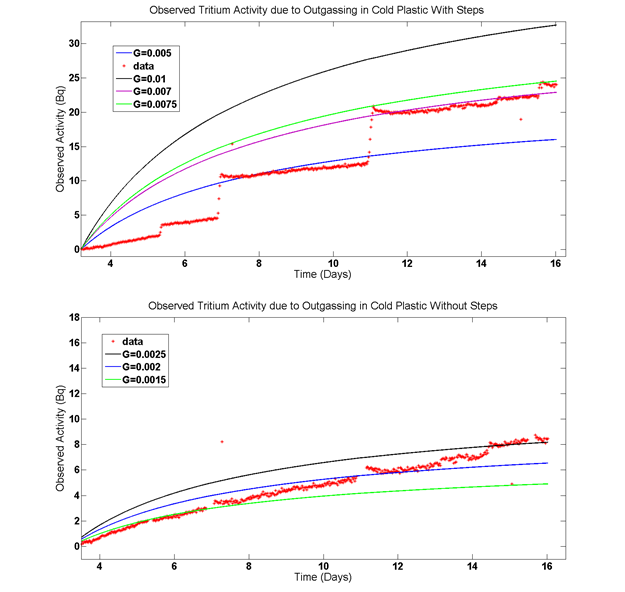
\includegraphics[scale=0.85]{StepsandNoSteps.png}
\captionof{figure}{Top: A fit of the integral of the flux of CH$_3$T out of plastic over time using different values of $G$ to the out gassing data collected in Maryland's liquid xenon system assuming that the step features are due to diffusion.  This fit is used to set an upper limit on $G$.  Bottom: A fit of the integral of the flux of CH$_3$T out of plastic over time using different values of $G$ to the out gassing data collected in Maryland's liquid xenon system assuming that the step features are not due to diffusion.  This fit is used to set a lower limit on $G$. }
\end{center}

With a constraint on $G$ taken from the analytic solution to Fick's second law, we turn to numerical simulation to answer the question of how much initial CH$_3$T activity to inject into LUX to meet our calibration conditions.  Several assumptions are made to simplify the numerical model.  First, we approximate the diffusion into plastic as being a one dimensional process. In three dimensions, Fick's laws are
\[J=-D\nabla \phi\]
\[\frac{\delta\phi}{\delta t} = D \nabla^2 \phi .\]
In cylindrical coordinates, these equations become
\[J = -D (\frac{\delta \phi}{\delta r} \vec{r} + \frac{1}{r}\frac{\delta \phi}{\delta \theta}\vec{\theta} + \frac{\delta \phi}{\delta z}\vec{z})\]
\[\frac{\delta \phi}{\delta t} = D ( \frac{\delta^2\phi}{\delta r^2} + \frac{1}{r}\frac{\delta \phi}{\delta r} + \frac{1}{r^2}\frac{\delta^2 \phi}{\delta \theta^2} + \frac{\delta^2 \theta}{\delta z^2}).\]
Since the plastic in our detector at Maryland and in LUX can be approximated by a cylindrical shell, there is no dependence on the azimuthal or $z$ coordinates.  Since $r$ is large compared to the thickness of the plastic shell, $\frac{\delta^2 \phi}{\delta r^2} \gg \frac{1}{r} \frac {\delta \phi}{\delta r}$, so we can make the approximations
\[J=-D\frac{\delta \phi}{\delta r}\vec{r}\]
\[\frac{\delta \phi}{\delta t} = D \frac{\delta^2 \phi}{\delta r^2}.\]  We assume the concentration of CH$_3$T in LUX is uniform throughout its volume.  This assumption is justified, since the design of LUX creates currents which stir the liquid xenon.  With perfect mixing the effect of the purifier can be modeled by adding an exponential time dependence to the outer volume.  The time constant of this decay is equal to the time it takes xenon to recircculate through the LUX detector.

We use a simple implementation of the first order Euler method for our numerical simulations.  The finite difference approximations of Fick's two laws in one dimension are 
\[J_{i,j} = -D \frac{\phi_{i+1,j}-\phi_{i,j}}{\Delta x }\]
\[\phi_{i,j+1} = \phi_{i,j} + \Delta t (D \frac{\phi_{i+1,j} - 2 \phi_{i,j} + \phi_{i-1,j}}{\Delta x^2}),\]
where $i$ is the spacial index and $j$ is the time index.  To avoid divergent solutions, we must have
\[D \frac{\Delta t}{\Delta x^2} \leq \frac{1}{2}.\]
For effects to be propagated across $N$ spacial bins, $N$ time steps are required.  Therefore, the effective time resolution is
\[\Delta t_{effective} = \Delta t \times N_x.\]

The diffusion is simulated by setting the concentration at the boundary of the piece equal to $KC_{out}$, where $C_{out}$ is the concentration of CH$_3$T in the xenon.  This concentration is dependent on time according to
\[\frac{\delta C_{out}}{\delta t} = J_{out} \frac{A_{plastic}}{V_{xenon}}-\frac{C_{out}}{\tau},\]
where $A_{plastic}$ is the surface area of the plastic cylinder, $V_{xenon}$ is the total volume of xenon in the fiducial region, and $\tau$ is the time it takes for on full purification cycle.  The first term on the right of this equation models out gassing of CH$_3$T from the plastic cylinder, while the second term models removal of CH$_3$T through purification.  Using the first order Euler method, we arrive at an expression for $C_{out}$ given by
\[C_{j+1}=C_j + \Delta t [(J_{1,j}-J_{N_x,j})\frac{A_{plastic}}{V_{xenon}}-\frac{C_j}{\tau}].\]
The initial concentration is defined by dividing the desired injection activity by the volume of the fiducial region.  We choose $D = 2.3 \times 10^{-9} \frac {cm^2}{sec}$ such that the half-infinite boundary conditions in our diffusion model is valid, and combine this with our allowed range of values for $G$ to extract a value for $K$.  We find that for all $G$ values in our allowed range, an initial injection activity of 0.1 Bq results in 15,000 calibration events with the background rate returning to $<$ 5\% of its initial value in less than one month. (Figure 18)

\begin{center}
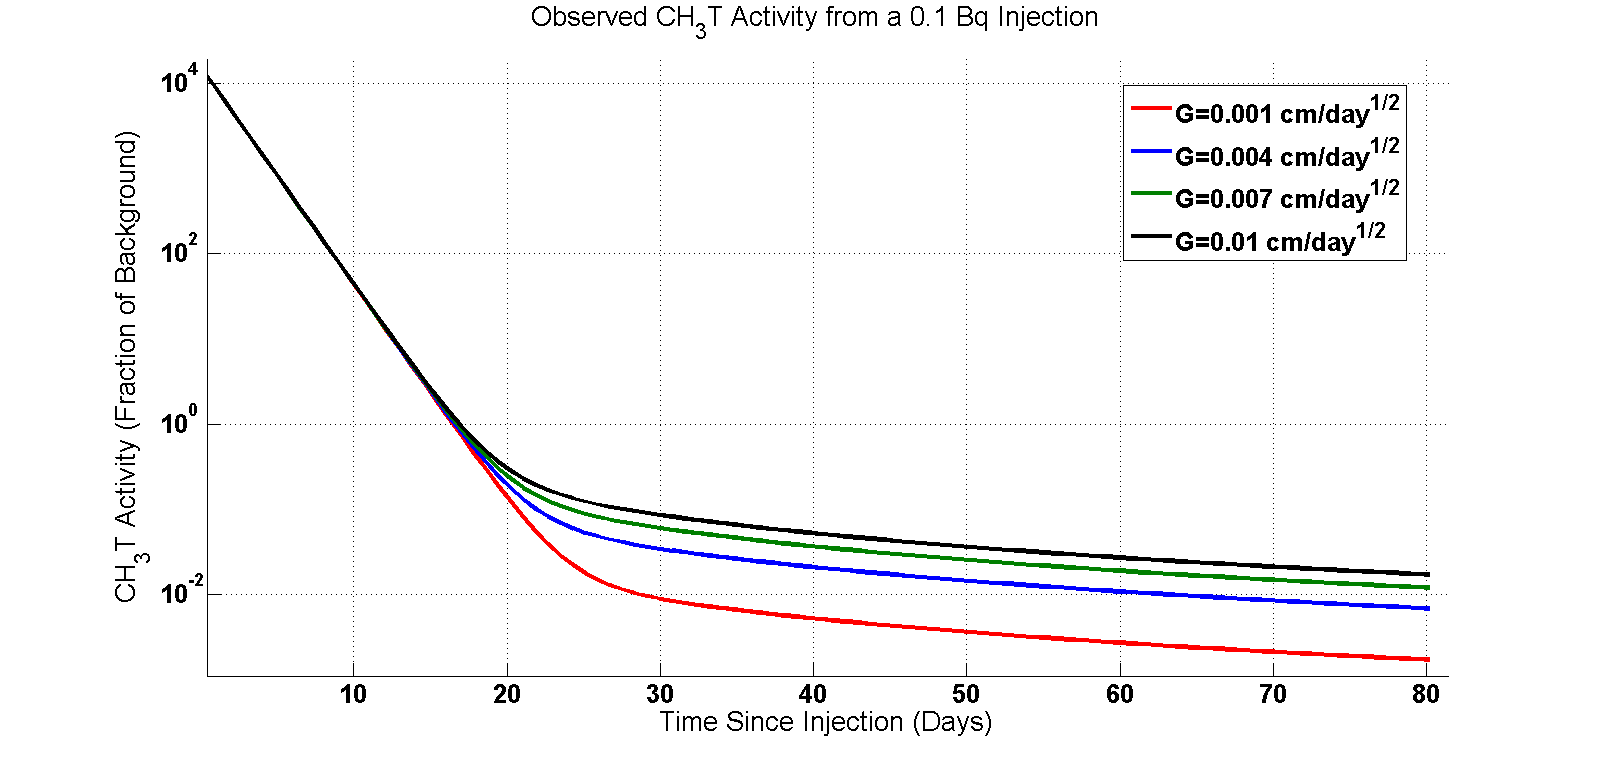
\includegraphics[scale=0.35]{LUXActivityOverTime.png}
\captionof{figure}{Simulated activity over time in LUX after a 0.1 Bq injection.}
\end{center}

\section{Tritium Injection System for LUX}

With the knowledge we obtained from our experiments at UMD we have designed and built a tritium injection system for the purpose of calibrating the LUX detector.  This tritium injection system consists of a tritiated methane bottle, a methane purifier, and subsequent expansion volumes to fine tune the amount of activity being injected.  The tritiated methane bottle contains a mixture of 35 becquerels of tritiated methane and 1400 torr of dekryptonated xenon gas.  The dekyrpotonated gas is included in the bottle to raise its pressure and ensure no backward flow from the LUX system into the bottle.  Multiple expansion volumes are included in the system so that a single injection can range from 0.00625 Bq to 0.4 Bq.  A pump-out port is built into the system so that the expansion volumes may be evacuated in preparation for subsequent injections.

\begin{center}
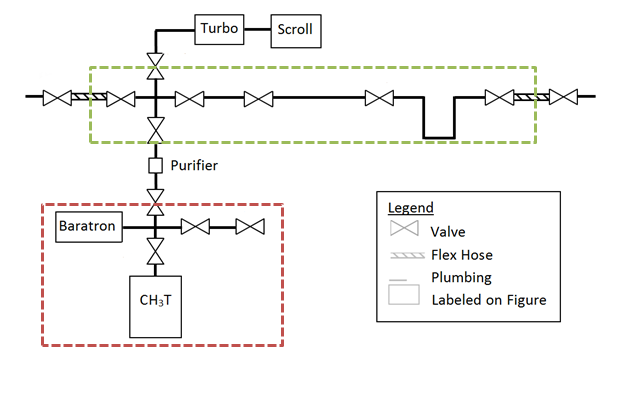
\includegraphics[scale=0.7]{Injection_Plumbing_Colored.png}
\captionof{figure}{A plumbing diagram of the CH$_3$T injection system for LUX.  The tritiated methane bottle and its corresponding pressure gauge is shown in red while the expansion volumes are shown in green. The purifier and pump out ports are labeled on the diagram.}
\end{center}

To use the system an operator must first determine which expansion volumes are required to obtain the desired injection activity.  Once these injection volumes have been filled with tritiated methane, the tritiated methane bottle is isolated and the LUX xenon gas flow is diverted through the expansion volumes.  This sweeps the tritiated methane out of the injection system and into the LUX detector.  Since LUX's standard operating mode has a xenon purifier included in its flow path this tritiated methane will be removed from the system as it circulates. 

LUX was designed such that no areas of stagnant gas should exist in the detector, making it unlikely to see residual contamination from pockets of unpurified CH$_3$T.  Using our diffusion simulations we have set a target injection activity of 0.1 bq for LUX.  This target injection activity should be adequately removed by our purifiers in less than 30 days.  Should our prediction prove to be wrong, the detector can be warmed to room temperature increase the out gassing rate of residual CH$_3$T in the plastics by a factor of $10^6$.

\section{Conclusion}

As the scale of dark matter detectors continues to grow, the importance of an internal electron recoil calibration source grows with it.  Using tritated methane injections into liquid xenon we have successfully developed such a source for use in dark matter detectors.  We find that a methane purifier is essential to remove impurities from the CH$_3$T source prior to any injection.  Once impurities in the CH$_3$T source has been removed, a hot zirconium getter can remove  100\% of any injected tritiated methane within our error bars.  Detector geometry and plastics surface area can result in residual contamination after a purification, and these effects must be modeled within each detector to ensure the successful calibration conditions are met.

\begin{thebibliography}{1}

\bibitem{Zwicky} Zwicky.  \emph{Helv. Phys. Acta} 6:110 (1933)
\bibitem{Persic} Persic, Salucci, Stel.  \emph{Mon. Not. R. Astron. Soc.} 281:27 (1996)
\bibitem{Battaner} Battaner, Florido.  \emph{Fund. Cosmic Phys.} 21:1 (2000)
\bibitem{Binney} Binney, Tremaine. \emph{Galactic Dynamics}. Princeton, NJ: Princeton Univ. Press (1988)
\bibitem{Javorsek} Javorsek II, Fischbach. \emph{The Astrophysical Journal} 568:1-8 (2002)
\bibitem{EROS} EROS Collab.  \emph{Astron. Astrophys.} 400:951 (2003)
\bibitem{Alcock} Alcock, et al. (MACHO collab.)  \emph{Ap. J.} 542:281 (2000)
\bibitem{Tytler} Tytler, et al. \emph{Ap. J.} 617:1-28 (2004)
\bibitem{Spergel} Spergel, et al. \emph{Ap. J. Suppl.} 148:175 (2003)
\bibitem{Robertson} Robertson. \emph{J. Phys.:Conf. Ser.} 173:012016 (2009)
\bibitem{Parke} Parke.  \emph{FERMILAB-CONF-06-248-T} (2006)
\bibitem{Pastor} Pastor.  \emph{Physics of Particles and Nuclei} 42(4):628-640 (2012)
\bibitem{Kolb} Kolb, Turner. \emph{The Early Universe}.  Cambridge, MA: Perseus (1994)
\bibitem{Jungman} Jungman, Kamionkowski, Griest.  \emph{Phys. Rep.} 267:195 (1996)
\bibitem{Goldberg} Goldberg.  \emph{Phys. Rev. Lett.} 50:1419 (1983)
\bibitem{Ellis} Ellis, et al. Nucl. \emph{Phys. B} 238:453 (1984)
\bibitem{Bennett} Bennett, et al. \emph{Ap. J. Suppl.} 148:1 (2003)
\bibitem{Arnowitt} Arnowitt, Dutta, Hu. \emph{Beyond The Desert '03}, Castle Ringberg, Germany (June 2003), hep-ph/0310103
\bibitem{Roszkowski} Roszkowski.  \emph{Pramana} 62:1 (2004) hep-ph/0404052
\bibitem{Baluni} Baluni. \emph{Phys. Rev. D} 19, 2227 (1979)
\bibitem{Chung} Chung, et al.  \emph{Phys. Rev. D} 59:023501 (1999) arXiv:hep-ph/9802238
\bibitem{Goodman} Goodman, Witten. \emph{Phys. Rev. D} 31:3059 (1985)
\bibitem{Lewin} Lewin, Smith. \emph{Astropart. Phys.} 6:87 (1996)
\bibitem{Shan} Shan. \emph{JCAP} 1107:005 (2011)
\bibitem{Gaitskell} Gaitskell.  \emph{Annu. Rev. Nucl. Part. Sci.} 54:315-359 (2004)
\bibitem{McKinsey} McKinsey, et al.  \emph{Journal of Physics: Conference Series} 203:012026 (2010) 
\bibitem{Fiorucci} Fiorucci, et al.  \emph{AIP Conference Proceedings} 1200:977 (2010)
\bibitem{Kastens} Kastens, et al. \emph{Phys. Rev. C} 80:045809 (2009)

\bibitem{D'Amico} D'Amico, Guido, et al. arXiv:0907.1912[astro-ph.CP] 
\bibitem{Wu} Wu, et al.  \emph{Monthly Notices of the Royal Astronomical Society} 301(3):861-971.  arXiv:astro-ph/9808179
\bibitem{Griest} Griest, et al.  \emph{Phys. Rept.} 333:167-182 (2000) 
\bibitem{Aprile} E. Aprile, T.Doke. \emph{Rev. Mod. Phys.} 82:2053-2097 (2010)
\bibitem{Miyake} Miyake, et al.  \emph{J. vac. Sci. technol. A.} 1:1446-1451 (1983)
\bibitem{Piche} R. Piche. \emph{Partial Differential Equations} Tampere University of Technology.



\end{thebibliography}


\end{document}

